\documentclass[11pt]{article}
% Packages
\usepackage{times}
\usepackage[fleqn]{amsmath}
\usepackage{amssymb}
\usepackage{anysize}
\usepackage{graphicx}
\usepackage{booktabs}
\usepackage{titlesec}
\usepackage{float}
\usepackage{natbib}
\usepackage[english]{babel}
\usepackage[autolanguage]{numprint}
\usepackage[tableposition=top]{caption}
\usepackage{subcaption}
\usepackage[colorlinks=true]{hyperref}
\usepackage{pgfplots}

% Macros
\newcommand{\np}{\numprint}
\newcommand{\tdl}{TD($\lambda$)}
\newcommand{\uid}[1]{\texttt{#1}}
\newcommand{\ab}{$\alpha$-$\beta$}

% Options
\pgfplotsset{%
  cycle list name=exotic,
  every axis legend/.append style={nodes={right}, font=\footnotesize},
  bar cycle list/.style={/pgfplots/cycle list={%
      {fill=teal},%
      {fill=orange},%
      {fill=cyan!60!black},%
      {fill=red!70!white},%
      {fill=lime!80!black},%
      {fill=red},%
      {fill=yellow!60!black},%
    }
  },
}
\marginsize{1cm}{1.5cm}{1cm}{1.5cm}

% Title spec
\title{%
  COMP3130 --- Group Project in Computer Science \\
  10$\times$10 Othello Learning Agent}
\date{June 8, 2012}
\author{%
  Andrew Haigh\thanks{\uid{u4667010}} \and %Neato.
  Timothy Cosgrove\thanks{\uid{u4843619}} \and
  Joshua Nelson\thanks{\uid{u4850020}}}

% Section styling
\titleformat{\section}%
  {\large\itshape}%
  {\thesection.}{.5em}{}%
  [\vspace{1ex}\titlerule]%
\titleformat{\subsection}%
  {\itshape}%
  {\thesubsection.}{.5em}{}%

% Document
\begin{document}
\maketitle
\begin{abstract}
  \label{abstract}
  An agent to play the board game Othello is created, with the ability
  to learn through reinforcement. The minimax algorithm is used for game
  playing, and a static evaluation function for the leaf nodes is learnt by
  self play.  The agent learns the insignificance of the number of stones, and
  the significance of stone positioning. This agent is played against itself,
  and against other developed agents, and its performance is analysed.
\end{abstract}
\clearpage

\section{Problem overview}
\label{sec:problem_overview}
%%Describe the game and the nature of the task
In this project we were tasked with the challenge of developing a learning
agent to play a variant of the game Othello. Othello is a two-player zero-sum
game traditionally played on an 8$\times$8 board with players alternately
placing stones so as to capture lines laid down by their opponent, reversing
the colour of the intermediate discs in the process.
In this variant the game will be played on a 10$\times$10 board with four
squares chosen to be blocked. Blocked squares cannot be played on or captured,
and they interrupt capture lines. These four squares are randomly determined at
the beginning of each match, and are not allowed to be one of the
locations of the four initial stones. These squares introduce a significant challenge
for the AI agent by since the board configuration will be different each match.
(making the use of pre-computed data difficult)

To this end, we were provided with a sample implementation of an Othello
server and simple client code in C++. Our subsequent task was to implement an
agent to generate the game tree for Othello from an arbitrary state to a
certain depth, evaluate these states using a static evaluation function, then
use minimax back-propagation to chose the most appropriate move which it would
then communicate to the server.

\section{Solution overview}
\label{sec:solution_overview}
%%A minimax agent with a static evaluation function.
Our client is broken into various logical interfaces: a client which handles
communications, board methods which handle state space calculations, a player
which chooses its next best move given the current state of the game, and
features which evaluate the strength of arbitrary game states.

%Wrote this for Static eval but realised it should go here in the explanation
%of minimax
The state space for our modified othello game is exceedingly large
(approximately $3^{92}$ or $7 \times 10^{43}$ possible states) and while some
of these states are unreachable or duplicates it is obviously impossible to
search the entire space every turn. So at some point we must cut off the
search and apply a static evaluation function.

%%I feel as though these should be sub-headings. feel free to change back if disagree
\subsection{Optimisations}
\label{sub:optimisations}
%% Alpha beta pruning, negamax, etc.
Our agent went through numerous incremental improvements towards our final
competition submission. After implementing basic communications code a basic
implementation was created for generating subsequent board states and then
simple greedy and minimax players were written into the client. Following
this \ab\ pruning was implemented, providing a performance increase over
naive minimax by eliminating some subtrees of the game-tree which do not
affect the overall minimax values.
% Include a description of how alpha-beta pruning works here
Finally, the \ab\ implementation was
changed to a Negamax implementation, taking advantage of the adversarial
nature of the game. This rests on the fact that for real numbers
\[
  \max(\alpha, \beta) = -\min(-\beta, -\alpha).
\]
Though this provided negligble performance increase, it
reduced corner cases and made understanding player code easier.

After doing this, a simple heuristic was added in an attempt to increase
cutoffs. In essence, by guessing moves closest to the principal variation
(perfect play) more \ab\ cutoffs would be likely, increasing search speed.
Simple aggressive move ordering was added, ordering the first $n$ plies by the
number of pieces captured.

\subsection{Static evaluation function}
\label{sub:eval_func}
%% Necessity of a static evaluation function, features used, etc
As mentioned above, we have needs of a \emph{static evaluation function} which
evaluates the quality of state once we have searched to our depth cut-off.
This is implemented in Jafar by way of the FeatureSet class. This class keeps
track of a set of Feature objects; each with the ability to read in a board and
return some measure state quality.

The board features implemented by Jafar are:
\begin{center}\begin{tabular}{l l}
\textbf{Stone Count} & Number of stones on the board owned by the player\\
\textbf{Legal Moves} & Number of playable positions available; a measure of \emph{mobility}\\
\textbf{Blocked Adjacent} & Number of player owned squares adjacent to a blocked square\\
\textbf{Corner Pieces} & Number of corner squares owned by the player\\
\textbf{Side Pieces} & Number of edge squares owned by the player\\
\end{tabular}\end{center}
The last 3 features in this list all relate to \emph{stability}; encouraging the
agent to capture squares which are more easily protected.

Early in the development of Jafar we had one extra board feature:
\begin{center}\begin{tabular}{l l}
\textbf{Visibility} & Amount of empty space in a line from each of the player's stones\\
\end{tabular}\end{center}
but this feature proved to be a very poor performance measure as squares with a high
visibility were easy to capture. Furthermore the feature was costly compute
so was fully cut (rather than included at low or negative weight).

To obtain the final score of a state the FeatureSet normalises and weights the
above features and calculates a weighted sum. With normalisation this sum will lie
between 0 and 1 and corresponds to an approximation of the probability of winning from this state.

A challenge remains in determining the feature weights; i.e. how important each
feature is. To learn these weights in a formal sense we must build a learning algorithm.
Before this however we created some charts (Figure~\ref{fig:triangle1} and ~\ref{fig:triangle2})
to visualise the feature space, providing a preliminary view of what our learning algorithm will find as the optimal weights.

\begin{figure}[H]
  \centering
   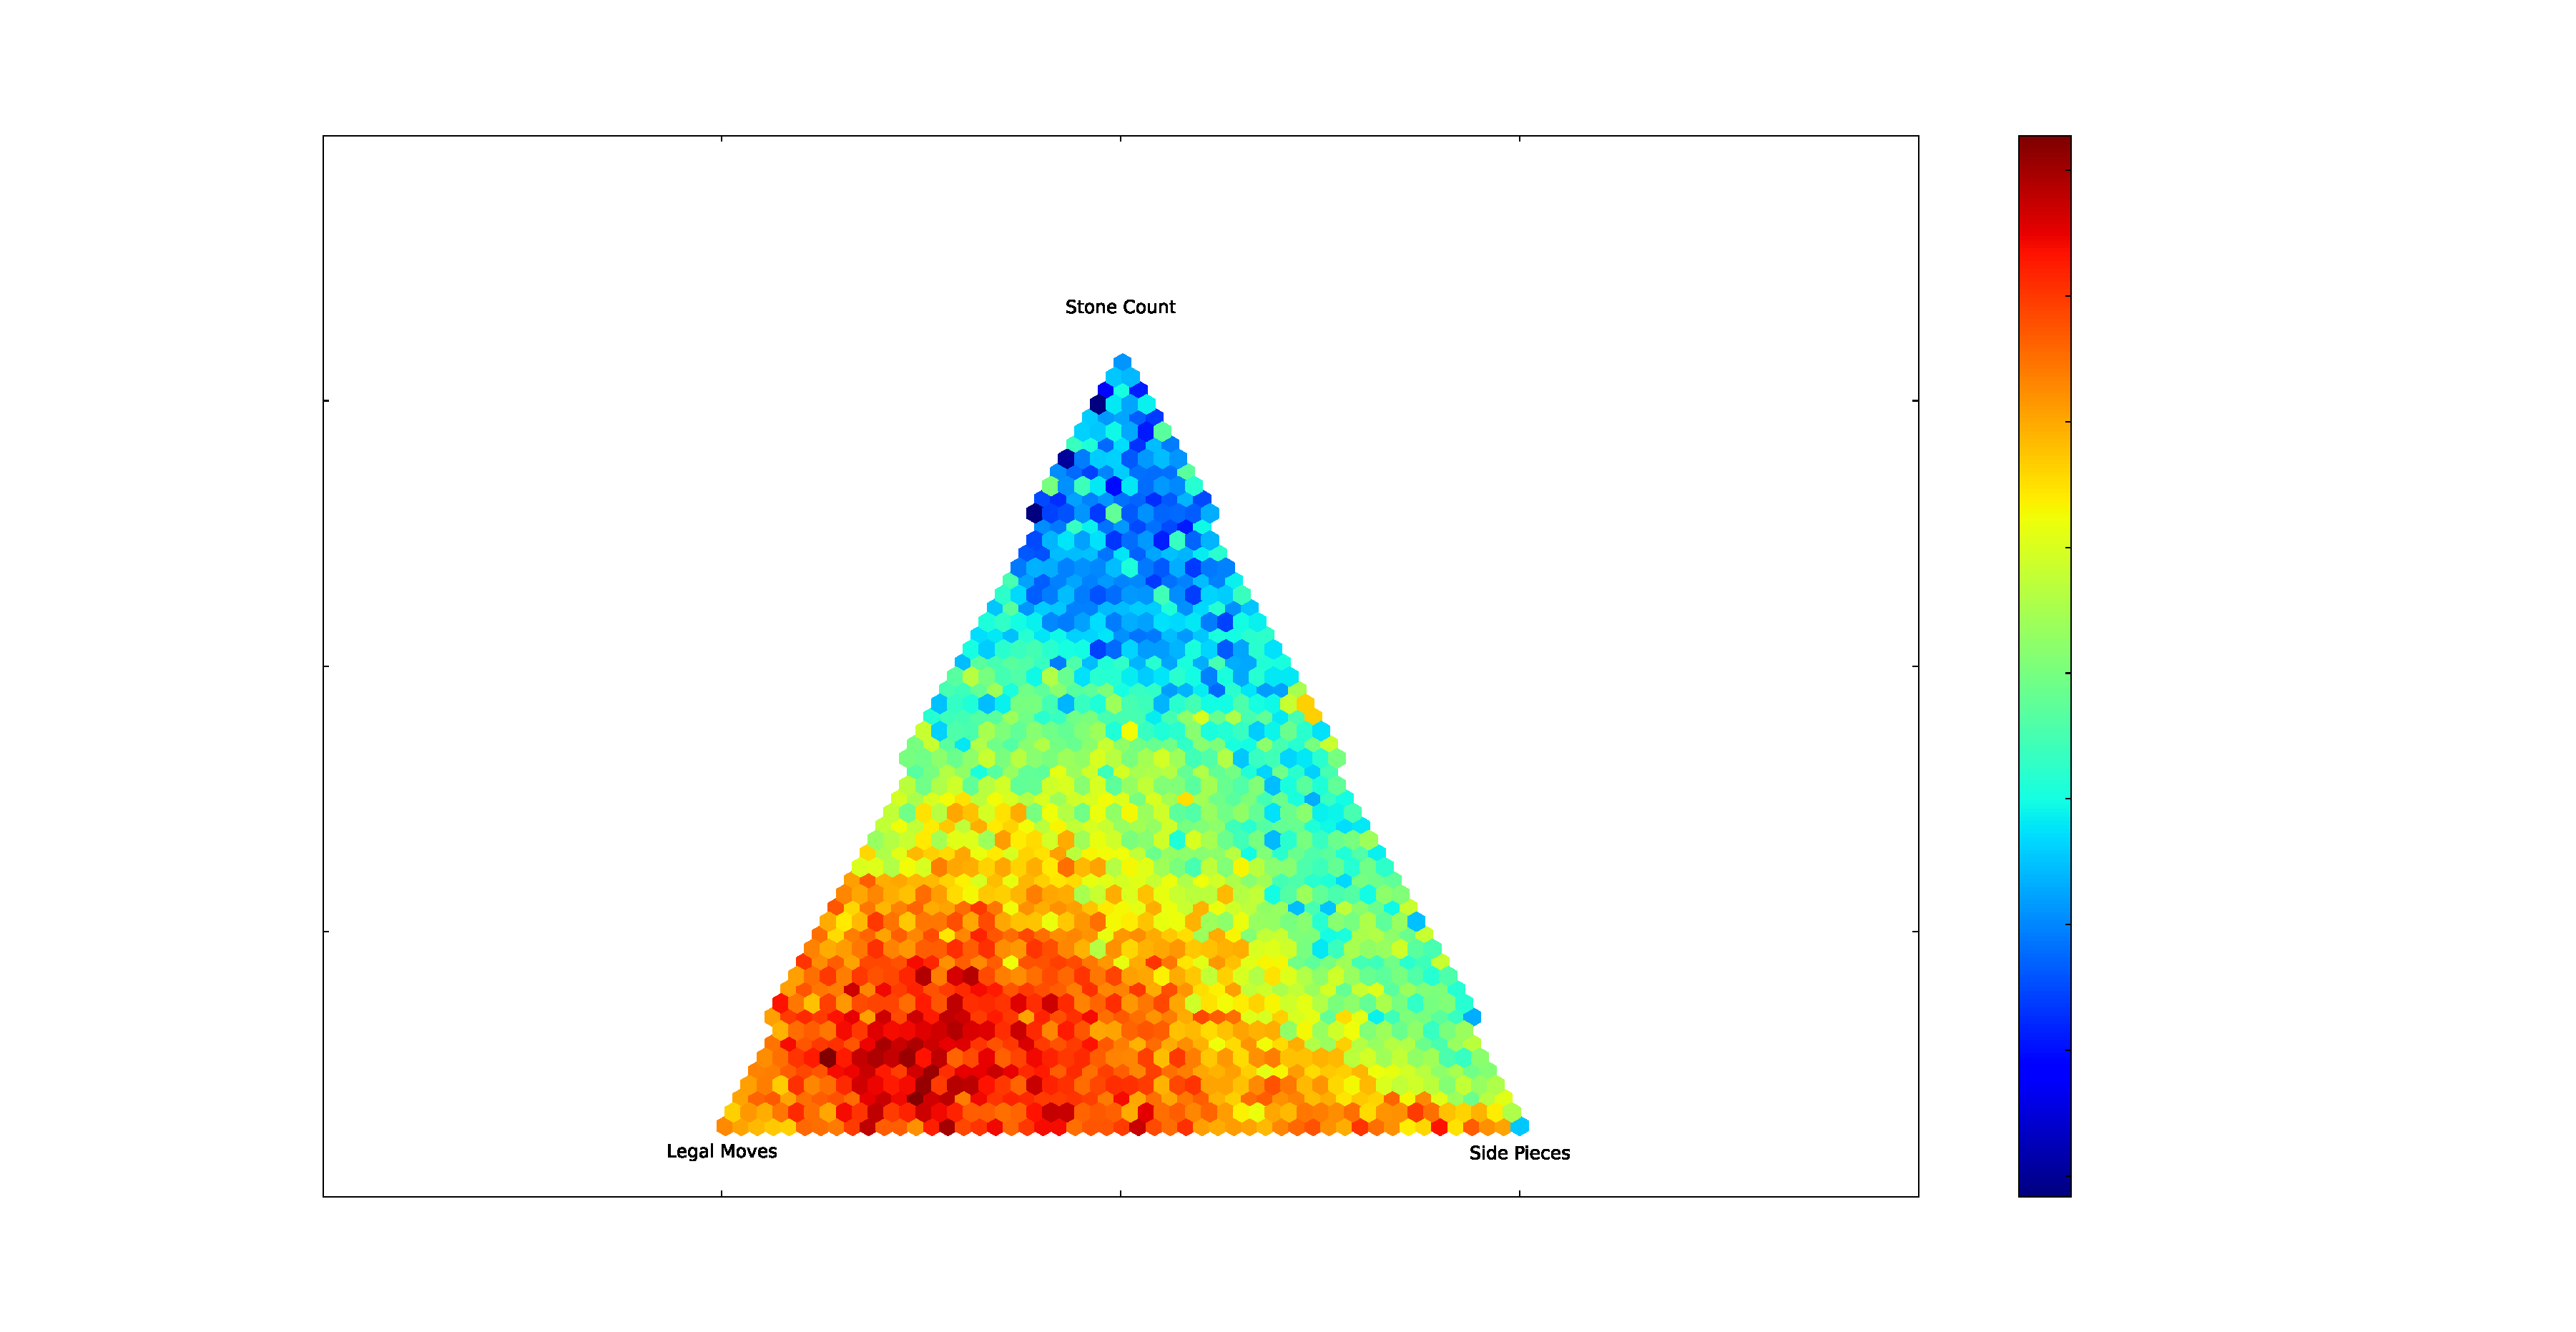
\includegraphics[trim= 12cm 4.45cm 23cm 8cm, clip, height=8cm]{../Graphs/LegalMoves_Count_SidePieces_Triangle.pdf} 
  \caption{Weight Space for LegalMoves (left), SidePieces (right) and StoneCount (top)}
  \label{fig:triangle1}
\end{figure}

\begin{figure}[H]
  \centering
  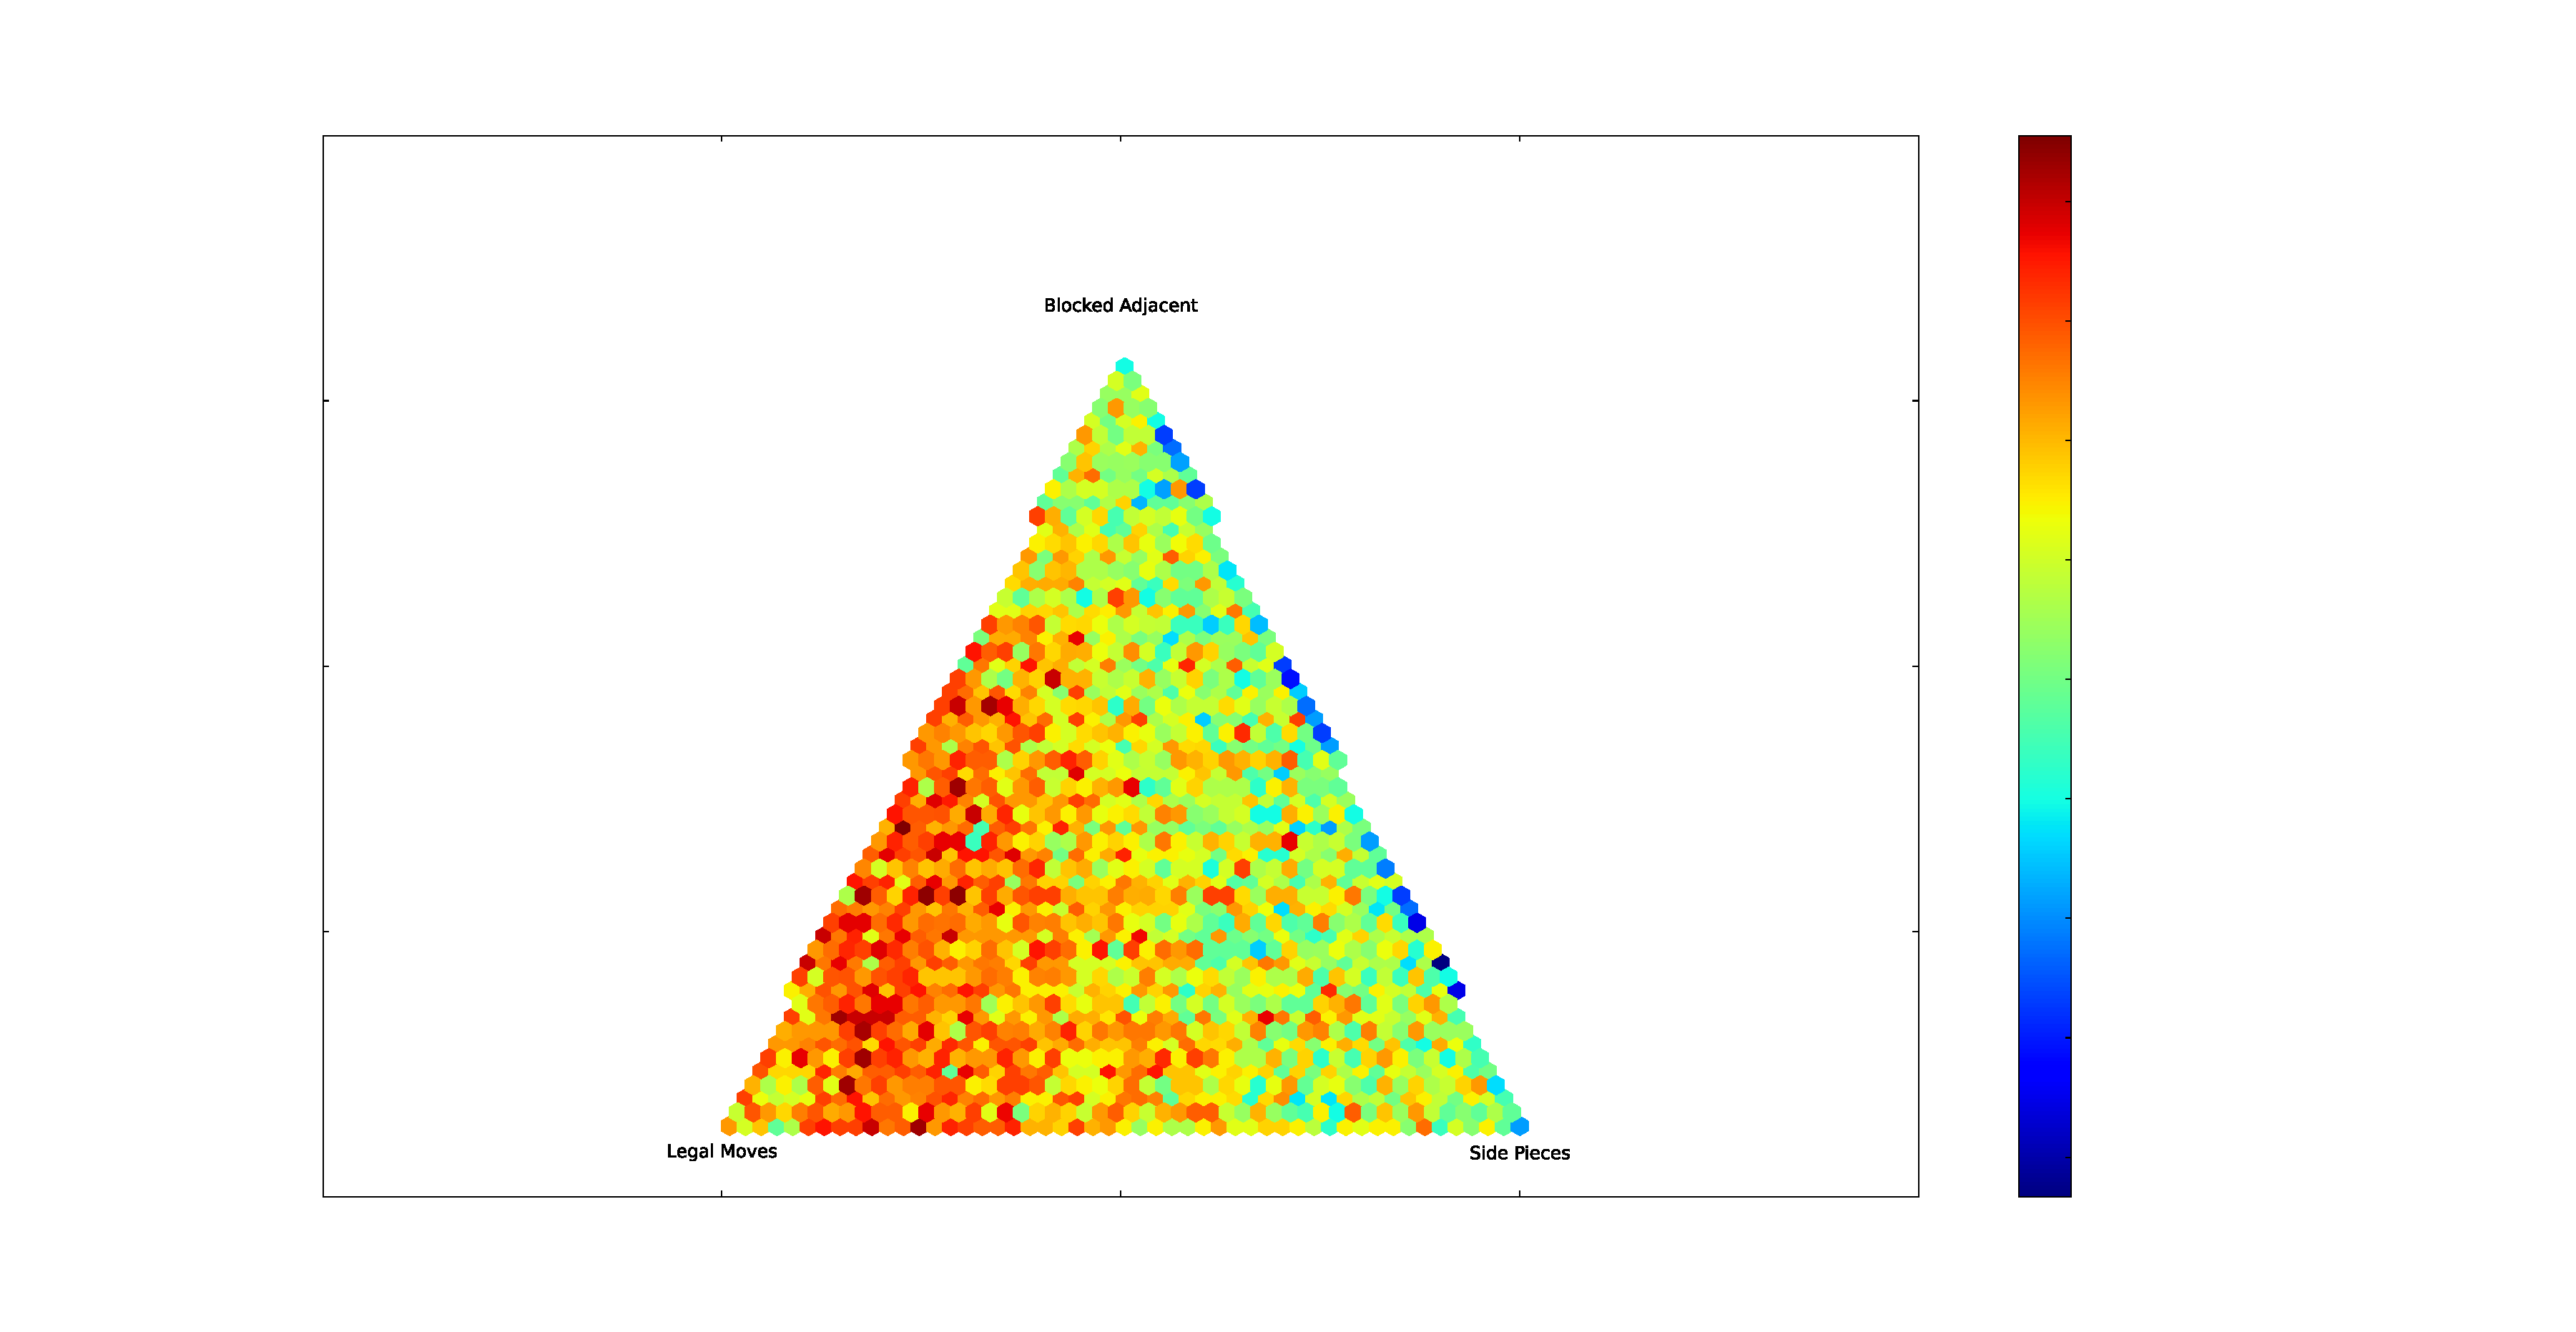
\includegraphics[trim= 12cm 4.45cm 23cm 8cm, clip, height=8cm]{../Graphs/LegalMoves_BlockedAdjacent_SidePieces_Triangle.pdf} 
  \caption{Weight Space for LegalMoves (left), SidePieces (right) and BlockedAdjacent (top)}
  \label{fig:triangle2}
\end{figure}

Each point on the charts above represent an agent with feature weights corresponding to
how close the data point is to each corner of the triangle. The colour intensity of the data
point describes the agent's win rate against a generic Negamax player; using only StoneCount
to evaluate states. These win rates range from 100\% (deep red point) to about 40\%(deep blue point).

In the first graph we see very clearly defined boundaries; showing that ideal weightings
put priority on LegalMoves and SidePieces before StoneCount. The second graph is less
clearly defined but we still see an overall trend that LegalMoves and BlockedAdjacent
take precedence over SidePieces.

\section{Learning}
\label{sec:learning}

We have provided a visual overview of what features will be weighted higher
than others, and now our next task becomes that of implementing a learning algorithm
to formally learn the optimal feature weights; providing us the with
the strongest play. We considered and implemented two strategies for learning
these weights: Temporal Difference learning as \tdl, and a genetic algorithm
using Elo scores as a fitness metric.

\subsection{\tdl}
\label{sub:tdlambda}

The \tdl\ algorithm was used to learn the weighting of the static evaluation
function's various features. \tdl\ was first described by \citet{Sutton1988}
in his seminal paper on the topic. The implementation of this algorithm is
based on the one implemented by the KnightCap agent as described by
\citet{Baxter1997}.  At the end of each game played, the agent adjusts its
weights according to the following formula:

\begin{center}

    $\displaystyle w := w + \alpha \sum _{t=1} ^{N-1} \Delta \tilde{J}(x_t,w) \: \times \: \Big[ \sum ^ {N-1} _{j=t} \lambda^{j-t} d_t \Big] $\\
        
    \begin{tabular}{  l l | l l }
      $w$                   & The vector of weights                         &$x_t$  & The $t^{th}$ board in the game \\
      $\alpha$              & The learning rate                             &$\lambda$      &The discount factor \\
      $N$                   & The number of states in the game              &$d_t$          &$\tilde{J}(x_{t+1},w) - \tilde{J}(x_t,w)$\\
      $\Delta \tilde{J}$    & The derivative of the $\tilde{J}$ function    &               &\\
    \end{tabular}
\end{center}

In the above formula, the $\tilde{J}$ function estimates the probability of
winning from a given state, given a set of weights for features and our board.
It approximates the $J$ function, \\

\begin{center}
$
J(x_t) = \begin{cases} 1, & \mbox{if } x_t\mbox{ is a winning state} \\ 0, & \mbox{if } x_t\mbox{ is a lost state} \end{cases}
$
\end{center}

For each game state $x_t$, we adjust the weights according to a factor $d_t$,
which is the temporal difference. $d_t = \tilde{J}(x_{t+1},w) -
\tilde{J}(x_t,w)$, and the weight adjustment is scaled with this amount. The
key observation is, for the true $J$ function, $J(x_{t+1}) - J(x_t) = 0$, so
we adjust our weights relative to this amount.

From Figure~\ref{fig:learned_j}, we can see that the
$\tilde{J}$ function, while not accurate for the entirety of the game, is able
to predict the results within the last 20 moves. In comparison,
Figure~\ref{fig:initial_j} indicates that the $\tilde{J}$ function
initially is a bad approximation, as even after losing a game, the estimated
probability of winning is high.

\begin{figure}[htbp]
  \begin{subfigure}{0.45\textwidth}
    \centering
    \begin{tikzpicture}
      \begin{axis}[width=\linewidth,
          xlabel=Move,
          ylabel=$\tilde{J}$,
          enlargelimits=false,
          ymin=0, ymax=1]
        \addplot+[mark=none] table[x=move, y=J]
          {../Graphs/JFunction_Data/iteration1_lost.txt};
      \end{axis}
    \end{tikzpicture}
    \caption{Losing a game}
  \end{subfigure}
  \hspace{1em}
  \begin{subfigure}{0.45\textwidth}
    \centering
    \begin{tikzpicture}
      \begin{axis}[width=\linewidth,
          xlabel=Move,
          ylabel=$\tilde{J}$,
          enlargelimits=false,
          ymin=0, ymax=1]
        \addplot+[mark=none] table[x=move, y=J]
          {../Graphs/JFunction_Data/iteration1_won.txt};
      \end{axis}
    \end{tikzpicture}
    \caption{Winning a game}
  \end{subfigure}
  \caption{$\tilde{J}$ Function initially}
  \label{fig:initial_j}
\end{figure}

\begin{figure}[htbp]
  \begin{subfigure}{0.45\textwidth}
    \centering
    \begin{tikzpicture}
      \begin{axis}[width=\linewidth,
          xlabel=Move,
          ylabel=$\tilde{J}$,
          enlargelimits=false,
          ymin=0, ymax=1]
        \addplot+[mark=none] table[x=move, y=J]
          {../Graphs/JFunction_Data/iteration1000_lost.txt};
      \end{axis}
    \end{tikzpicture}
    \caption{Losing a game}
    \label{fig:learned_j_lost}
  \end{subfigure}
  \hspace{1em}
  \begin{subfigure}{0.45\textwidth}
    \centering
    \begin{tikzpicture}
      \begin{axis}[width=\linewidth,
          xlabel=Move,
          ylabel=$\tilde{J}$,
          enlargelimits=false,
          ymin=0, ymax=1]
        \addplot+[mark=none] table[x=move, y=J]
          {../Graphs/JFunction_Data/iteration1000_won.txt};
      \end{axis}
    \end{tikzpicture}
    \caption{Winning a game}
    \label{fig:learned_j_win}
  \end{subfigure}
  \caption{$\tilde{J}$ Function after 1000 learning iterations}
  \label{fig:learned_j}
\end{figure}

In Figure \ref{LearningProgress}, we can see the progress of the learning
agent as it plays against a fixed opponent. After about 1000 games, the agent
settles on a win/loss ratio of approximately 0.7. 
%The weights learnt were
%split into 20 stages. Figure \ref{WeightsOverTime} shows the how highly the
%various features are weighted as a game progresses. We see that the `Legal
%Moves' feature is weighted highly early in the game, and later in the game,
%valued less. On the other hand, corner pieces and side pieces become more
%important as we approach the mid and end game. This makes sense, as the number
%of legal moves on the board is limited later in the game, and it is unlikely
%that a side or corner piece will be taken in the first quarter of the game.



\begin{figure}[htbp]
  % Currently the formatting of these graphs are terrible. I have no idea how
  \centering
  % it can be fixed though unfortunately. Little better... J functions show it up now though
  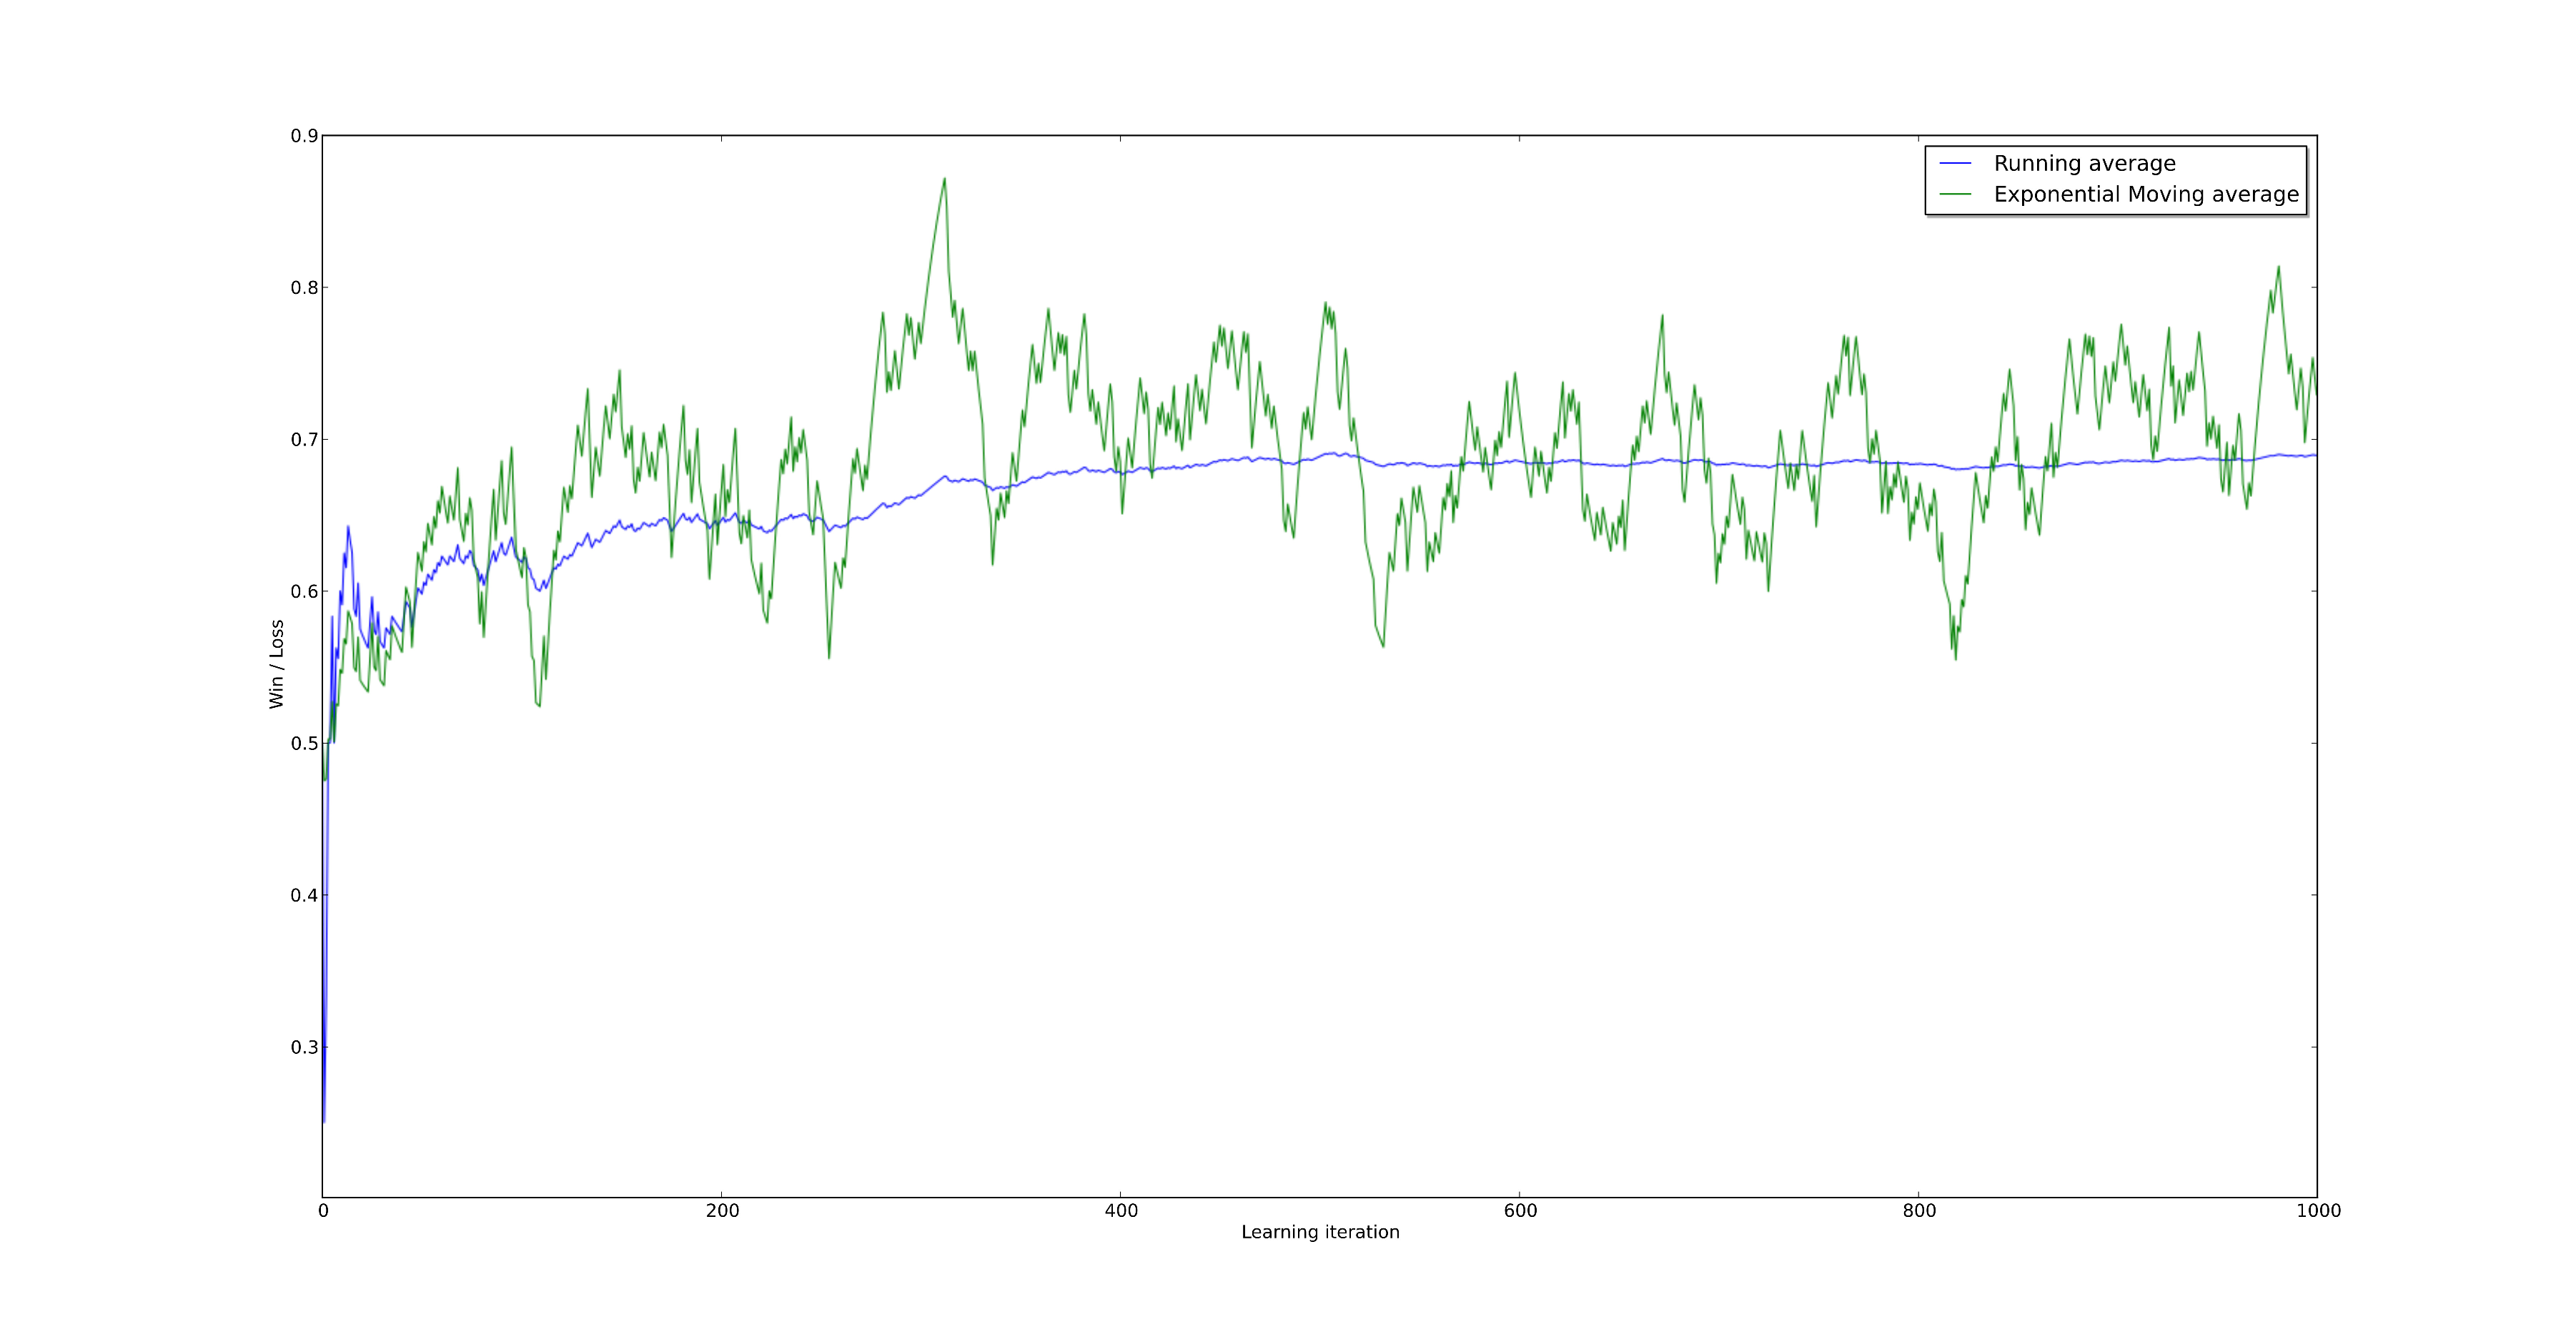
\includegraphics[trim= 6cm 2cm 5.5cm 3cm, clip,width=1\textwidth]{../Graphs/Learning_2ply_First1000.pdf}
  \caption{Learning Progress of a 4-ply Learning player vs. a 4-ply Minimax
    player}
  \label{LearningProgress}
\end{figure}

\subsection{Staged Learning}
\label{sec:staging}

Jafar performs \tdl\ learning in \emph{stages}. Each stage defines a separate
set of feature weights for a certain number of moves in the game. This allows
the agent to play with alternate strategies at different points throughout the
game, for example playing conservatively and leaving options open early game
and changing to a greedier nature near the end.

At the time of the competition our staged learning code was still highly 
experimental; as such the competition version of Jafar only contains weights learnt
over 3 stages. Below we see another agent with learning performed to 20 stages; 
and in the most extreme case we can split the agent into 92 game stages, maintaining a different set of
feature weights for every move of the game.

However, each stage we add to the agent corresponds to a linear increase in
the number of parameters \tdl\ must learn. This possibly leads to an
exponential increase in convergence time for the algorithm.  In
Figure~\ref{WeightsOverTime} and Figure~\ref{WeightsOverTime92} below we see
show the feature weights throughout the game for a 20-stage and 92-stage
version of Jafar; with \tdl\ run over 1000 and 30000 games respectively.

Notice that the two graphs are for the most part very similar; we see all the
same trends in both (though the 92-stage agent shows these trends in greater
detail). Note that the 20-stage agent has been running for a thirtieth the
amount of time that the 92-stage agent has; and the fact that the results are
similar reflects our above intuition regarding the increase in learning time
required.

Both agents below exhibit excessive `zig-zagging' (more notably in the
92-stage agent). This effect occurs due to the \emph{parity} of the board:
optimal play style differs slightly depending on whether or not the
agent will take the last move of the game. This effect is still observable in
the 20-stage agent since the stages have a differing amount of odd and even
parity moves.

%Hrmmmm looks good but really needs to be consistent with 92-stager. So need to
%rollback or tikzify both (or could fix colours here and axes below?)
\begin{figure}[htbp]
  \centering
  \begin{tikzpicture}
    \begin{axis}[width=0.75\textwidth, height=0.5\textwidth,
      xlabel=Stage, ylabel=Feature Weight, legend columns=2,
      ytick={0, 0.1, 0.2, 0.3, 0.4, 0.5},
      no markers, enlargelimits=false, ymin=0, ymax=0.5]
      \addplot table[x=stage, y=LM] {../Graphs/Weights_Over_Time_20.txt};
      \addlegendentry{Legal Moves}
      \addplot table[x=stage, y=SC] {../Graphs/Weights_Over_Time_20.txt};
      \addlegendentry{Stone Count}
      \addplot table[x=stage, y=BA] {../Graphs/Weights_Over_Time_20.txt};
      \addlegendentry{Blocked Adjacent}
      \addplot table[x=stage, y=SP] {../Graphs/Weights_Over_Time_20.txt};
      \addlegendentry{Side Pieces}
      \addplot table[x=stage, y=CP] {../Graphs/Weights_Over_Time_20.txt};
      \addlegendentry{Corner Pieces}
    \end{axis}
  \end{tikzpicture}
  \caption{Learned weights for a 20-stage player after 1000 learning
    iterations}
  \label{WeightsOverTime}
\end{figure}

\begin{figure}[htbp]
  \centering
  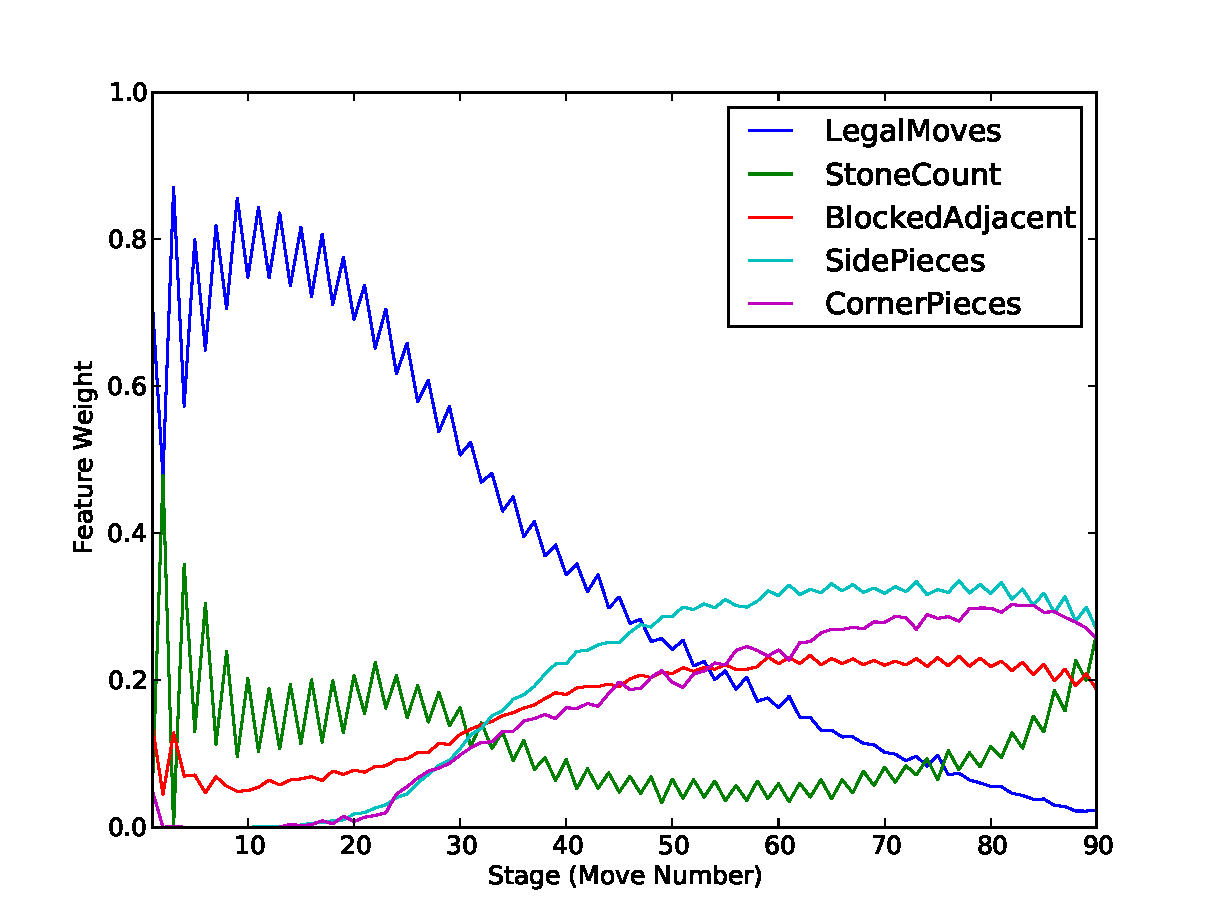
\includegraphics[trim=0cm 0cm 1.5cm 1cm, clip, width=0.75\textwidth]
    {../Graphs/finalweights.pdf}
  \caption{Learnt weights for a 92-stage player, after 30000 learning iterations}
  \label{WeightsOverTime92}
\end{figure}


\begin{figure}[H]
  \centering
  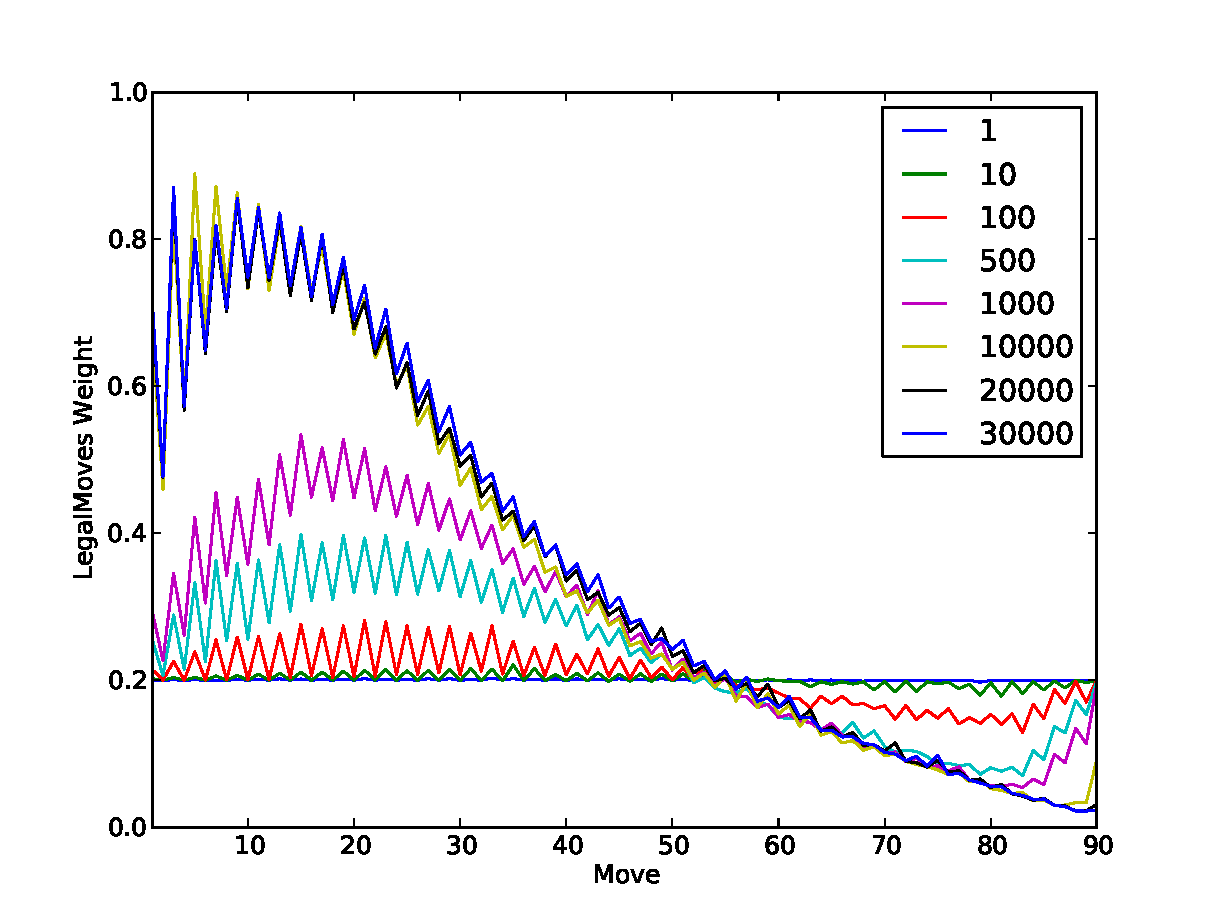
\includegraphics[trim=0cm 0cm 1.5cm 1cm, clip, width=0.75\textwidth]
    {../Graphs/legalmovesprogression.pdf}
  \caption{The LegalMoves feature weights converging over time}
  \label{LegalMovesConvergence}
\end{figure}

Figure~\ref{LegalMovesConvergence} shows us the convergence of the 92-stage agent
over time (for a single feature weight). Notice that there is very little
change after about 10000 games; implying that the agent has converged. Compare this
with the 20-stage agent above, who achieves a similar level of convergence after 1000
games.


\subsection{ELO Arena}
\label{sub:elo_arena}

While \tdl\ provides a exceedingly \emph{efficient} method of learning feature weights,
it is by no means \emph{intuitive}; in the sense that the learning process occurs
entirely within a mathematical formula. Thus we developed the \emph{ELO Arena};
a genetic algorithm entirely of our own design which serves to cross-validate
\tdl\ and more intuitively demonstrate learning.

The ELO Arena starts by generating a set of agents with random feature weights.
These agents then compete against each other for ELO rating points. The ELO rating
system was designed by Arpad Elo as a method of ranking international Chess players.
In the ELO Arena these rating points keep track of the relative skill levels of the competing
agents.

After each of the random agents have played a fixed number of games (and had their
ratings updated accordingly) a new agent is introduced. This new agent bases its feature
weights off of the current top 5 rated players in the following manner:
\begin{enumerate}
\item Take a weighted average of the feature weights from the top 5 players
\item \emph{Mutate} these weights by adding a random low-variance Gaussian variable
\end{enumerate}

Over time we should observe that agents with good mutations float to the top of the rating system.
This should lead to our new agents performing better and better until eventually
converging to weights similar to those learnt by \tdl.

\begin{figure}[htbp]
  \centering
  \begin{tikzpicture}
    \begin{axis}[width=0.75\textwidth, ybar, xlabel=Place, ylabel=Weight,
      enlarge y limits=false, enlarge x limits=0.12,
      ymax=0.55, ytick={0, 0.1, 0.2, 0.3, 0.4, 0.5}, xtick={1, 2, 3, 4, 5}]
      \legend{%
        Stone Count,
        Blocked Adjacent,
        Legal Moves,
        Side Pieces,
        Corner Pieces}
      \foreach \abbr in {SC, BA, LM, SP, CP}{
        \addplot table [y=\abbr] {../Graphs/ELOWinners.txt};
      }
    \end{axis}
  \end{tikzpicture}
  \caption{Feature weights for top 5 place getters in ELO Arena}
  \label{fig:elo_arena_weights}
\end{figure}

\subsection{Comparison of \tdl\ and ELO arena}
\label{sub:comparing_learning}
%% TD lambda and ELO arena

\begin{figure}[htbp]
  \centering
  \begin{tikzpicture}
    \begin{axis}[width=0.75\textwidth, ybar, xlabel=Stage, ylabel=Weight,
      enlarge y limits=false, enlarge x limits=0.12,
      ymax=1, ytick={0, 0.1, 0.2, 0.3, 0.4, 0.5, 0.6, 0.7, 0.8, 0.9},
      xtick=data, legend columns=-1]
      \legend{%
        Stone Count,
        Blocked Adjacent,
        Legal Moves,
        Side Pieces,
        Corner Pieces}
      \foreach \abbr in {SC, BA, LM, SP, CP}{
        \addplot table [y=\abbr] {../Graphs/ELOComparison.txt};
      }
    \end{axis}
  \end{tikzpicture}
  \caption{Comparison of ELO Arena winner vs.\ \tdl\ stage
    learner (ELO winner is stage 0)}
  \label{fig:elo_arena_comp}
\end{figure}

\section{Performance evaluation}
\label{sec:performance}
%% Tournament results, self play learning, fixed opponent results.
\begin{tabular}{c c c}
      & NegamaxPlayer at depth 2  & NegamaxPlayer at depth 4  \\
1-Stage Jafar at depth 2  & 0.61 & 0.43 \\ 
3-Stage Jafar at depth 2    & 0.70 & 0.44\\ 
92-Stage Jafar at depth 2   & 0.74 & 0.47\\
\end{tabular}
\section{Improvements}
\label{sec:improvements}
%% Look at the performance and say what we could have improved.
Many experimental features of Jafar were cut due to time constraints.

\subsection{Iterative Deepening}
\label{sub:i_deepening}

Iterative Deepening is a feature that was implemented at the time of the competition;
but was deemed too unstable and untested to be used in the agent.
It refers to the process of gradually increasing the depth at which Negamax searches to;
subject to some time constraint. This allows the agent to search deeper if
time is available or play conservative quick moves if we are running out of time.

In hindsight more time should have been spent on this feature. We see in the above results
(section ~\ref{sec:performance}) that a slight increase in depth corresponds to
a drastic increase in agent performance even where the static evaluation is poor.

\subsection{Generic Features}
\label{sub:generic_features}

A Generic Feature is a configuration of a small subset of the board which is
determined to be good for our overall position. The agent would have learnt these configurations
on its own over time; now being able to learn features uninfluenced from our human
perceptions of what is good.
Generic Features were our primary attempt at making use of pre-computed data despite
the inherit randomness in our modified game. Since it deals with small subsets of the
board we may still encounter configurations we know despite a different board as a whole.

This features proved difficult to implement; and would have taken an
extraodinary amount of time to learn and evaluate. Furthermore it is unlikely
that they would achieve a performance increase any more significant than a slight increase
in depth. Thus they were cut from Jafar
early in the development process.
\section{Final Comments}
\label{sec:final_comments}


\bibliographystyle{chicago}
\bibliography{ai}
\end{document}
